\section{{\gatekeeper}}
\label{sec:gatekeeper}

We already explained how to set up the initial {\gatekeeper} Administrator account in Section \ref{subsection:gatekeeper-admin}. This user is a {\gatekeeper} administrator, but does not have access permissions to any of your {\germinate} instances by default. Check Section \ref{sec:gatekeeper:permissions} to see how you can grant permissions to each user.

\subsection{Adding a new {\germinate} instance}
{\gatekeeper} can act as the authentication mechanism for as many {\germinate} instances as you like. By sharing the same {\gatekeeper} between multiple {\germinate} instances, you can reuse user accounts between instances.

Each time you want to add another {\germinate} instance that uses authentication to your system, you need to add it to {\gatekeeper} as well. By doing so, {\gatekeeper} knows about the {\germinate} instance and you can define which users should have access to the data.

\begin{figure}
	\centering
	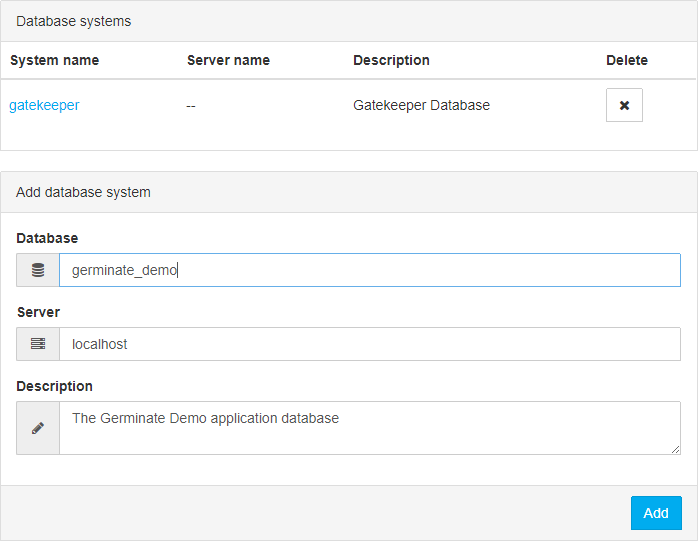
\includegraphics[width=0.8\textwidth]{img/gatekeeper/database-systems.png}
	\caption{The {\germinate} instance page lets you define {\germinate} instances. Each entry here represents a database schema. Specify the database server, database server and a description to define a new instance.}
	\label{fig:gatekeeper:instances}
\end{figure}

Figure \ref{fig:gatekeeper:instances} shows the interface that is used to define new {\germinate} instances. Each entry in the top table represents a {\germinate} database. Please note, that user access is based on the database, not the web-frontend and that it is indeed possible to have multiple web interfaces point at the same database. To define a new instance, fill in the text fields below the table and click on the "Add" button. The new instance will appear at the bottom of the table.

\subsection{Adding a new user}
To add a new user to the system, select "Add new user" in the main menu. Figure \ref{fig:gatekeeper:new-user} shows the interface that is used to add a new user. Fill in all the fields to create a new user. The user will automatically get limited access to {\gatekeeper} which allows them to change their email address and password easily.

\begin{figure}
	\centering
	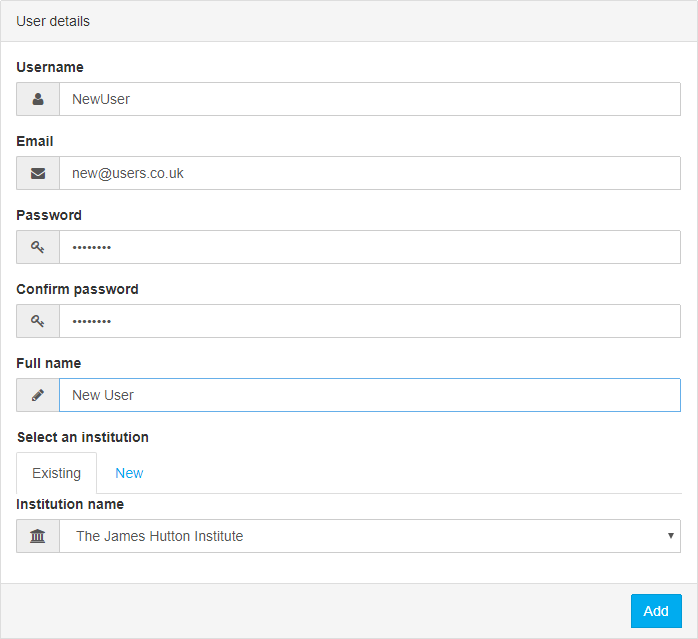
\includegraphics[width=0.8\textwidth]{img/gatekeeper/add-user.png}
	\caption{Adding a new user requires entering information about the user as well as setting a username and password.}
	\label{fig:gatekeeper:new-user}
\end{figure}

\subsection{Granting permissions}
\label{sec:gatekeeper:permissions}
There are two ways to grant permissions for a user to access a specific instance of {\germinate}. The first method involves selecting the user from the user list and then using the "Grant permission" section to add permissions to an existing {\germinate} instance or to grant permissions for a new instance.

For the second method, select the "View database system list" item in the main menu. Then select the system you want to add a user to. On the next page, use the form below the table to select the user and the user type to grant the new permission.

\subsection{Handling user registration requests}
If a {\germinate} instance allows users to register a new account, and this account needs to be approved before it can be used, an email will be sent to the main {\gatekeeper} email account informing the administrator that a new registration request is available.

Figure \ref{fig:gatekeeper:access-request} shows all the users that have requested access to an instance of {\germinate}. You can decide if you want to accept, reject or delete a request. Accepting the request grants the user access to the instance of {\germinate} and they will be able to view and download the data. Rejecting the user will remove the request and send an email to the user informing them that the request has been rejected. You can specify a specific reason for declining the request or just leave the text field blank. Deleting the request will just remove it from the list. No notification email is sent to the user.

\begin{figure}
	\centering
	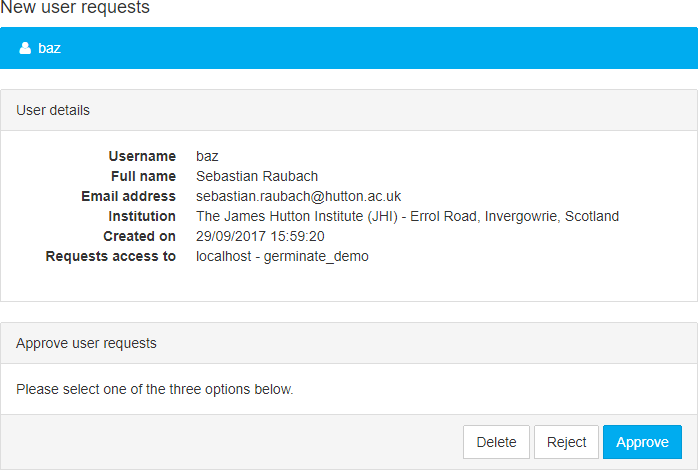
\includegraphics[width=0.8\textwidth]{img/gatekeeper/access-request.png}
	\caption{New users that await approval are shown under the "Approve users" menu item.}
	\label{fig:gatekeeper:access-request}
\end{figure}